\documentclass[compress]{beamer}
\usepackage{graphicx}
\usepackage{caption}

%gets rid of bottom navigation bars
\setbeamertemplate{footline}[frame number]{}

%gets rid of bottom navigation symbols
\setbeamertemplate{navigation symbols}{}

%gets rid of footer
%will override 'frame number' instruction above
%comment out to revert to previous/default definitions
\setbeamertemplate{footline}{}

\title{Generating Tree Genus Classification and Change Maps to Assist Mitigate Climate Change}
\author{Pedro Junio}
\date{\today}

\begin{document}

\frame{\titlepage}

\begin{frame}
\frametitle{Introduction}
\begin{itemize}
    \item Overview of tree genus classification
    \item Use of Sentinel-2 data and climate variables
    \item Objectives of the study
\end{itemize}
\end{frame}

\begin{frame}
\frametitle{Sentinel-2 Seasons}
\begin{itemize}
    \item Performance across different seasons
    \item Metrics: recall, precision, f1-score, PRC AUC, ROC AUC
    \item Optimal seasons for classification
\end{itemize}
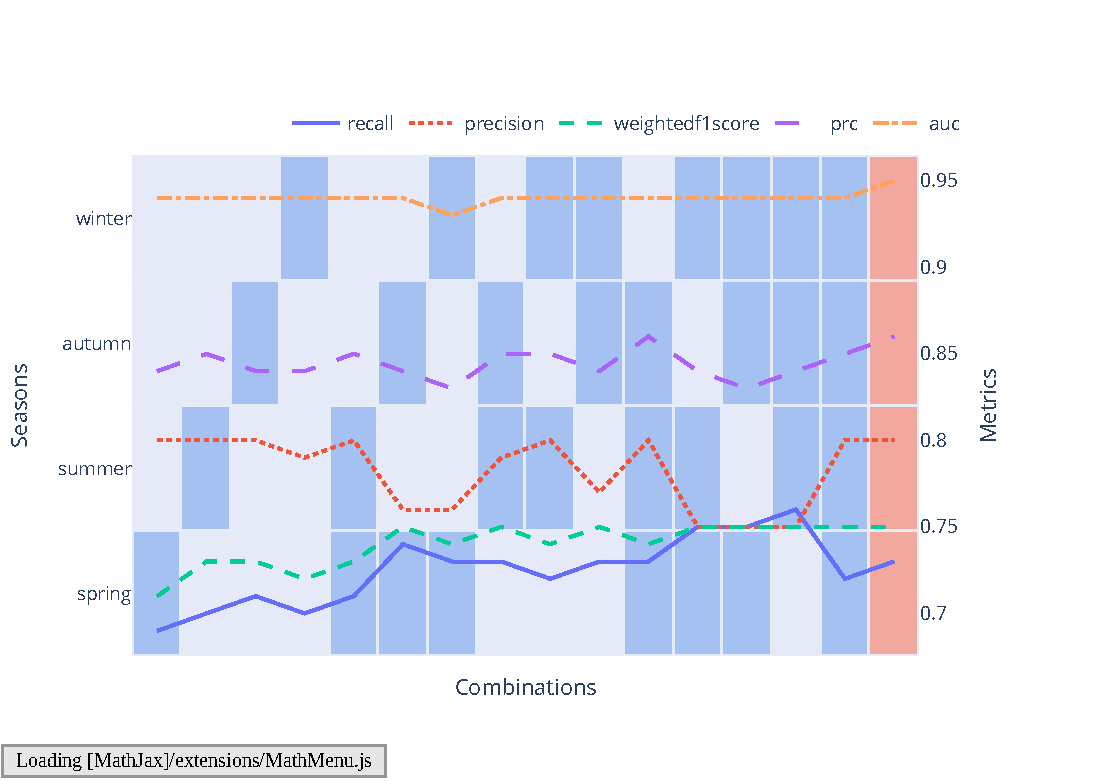
\includegraphics[width=0.9\linewidth, trim={20pt 40pt 10pt 30pt}, clip]{../report/figures/figures_analysis/seasonal_selection.pdf}
\end{frame}

\begin{frame}
\frametitle{Sentinel-2 Bands Part I}
\begin{itemize}
    \item Band selection and its impact on performance
    \item Analysis of band groups
\end{itemize}
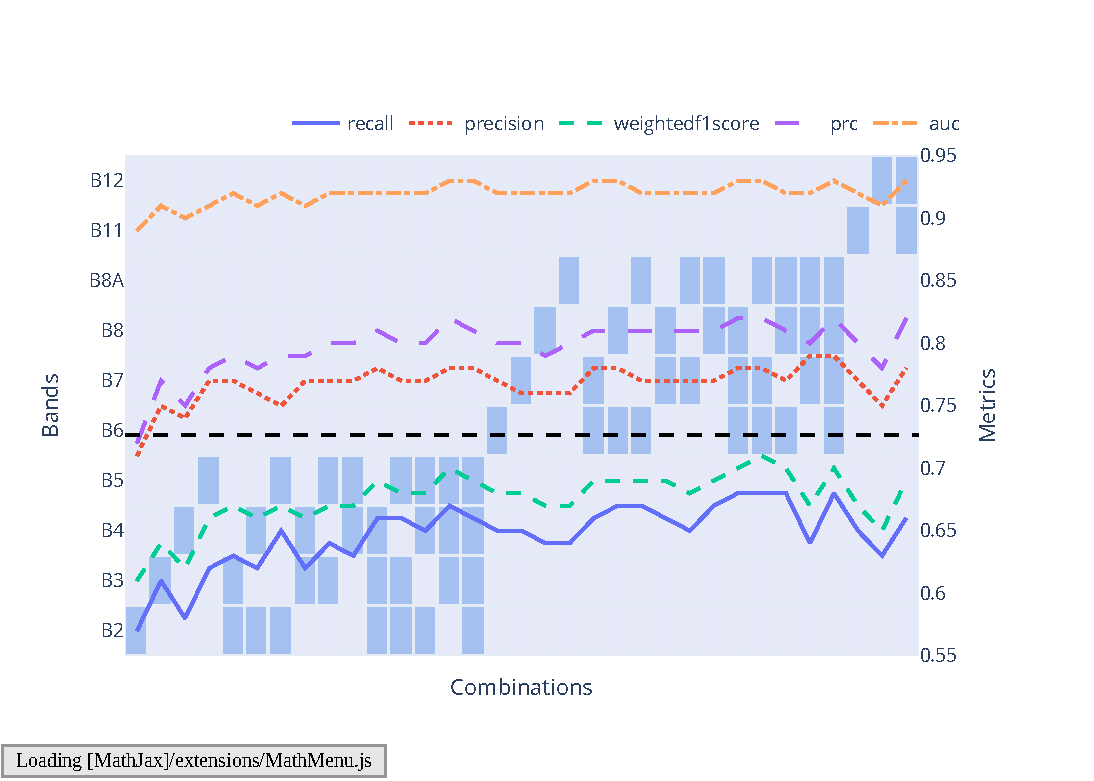
\includegraphics[width=0.9\linewidth, trim={20pt 40pt 10pt 30pt}, clip]{../report/figures/figures_analysis/band_selection.pdf}
\end{frame}

\begin{frame}
    \frametitle{Sentinel-2 Bands Part II}
    \begin{itemize}
        \item Optimal band combination for classification
    \end{itemize}
    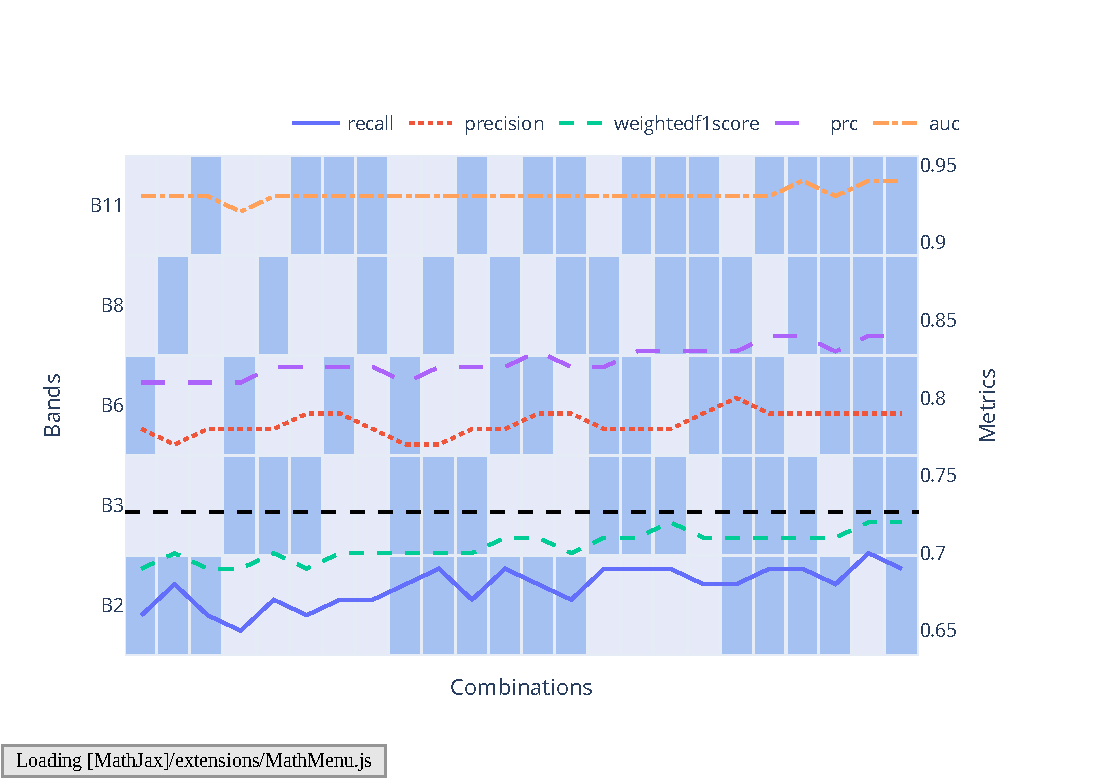
\includegraphics[width=0.9\linewidth, trim={20pt 40pt 10pt 30pt}, clip]{../report/figures/figures_analysis/band_selection_further.pdf}
    \end{frame}

\begin{frame}
\frametitle{Soil and Elevation Data}
\begin{itemize}
    \item Integration of SoilGrids and elevation data
    \item Performance comparison with Sentinel-2 data
    \item Impact on model accuracy
\end{itemize}
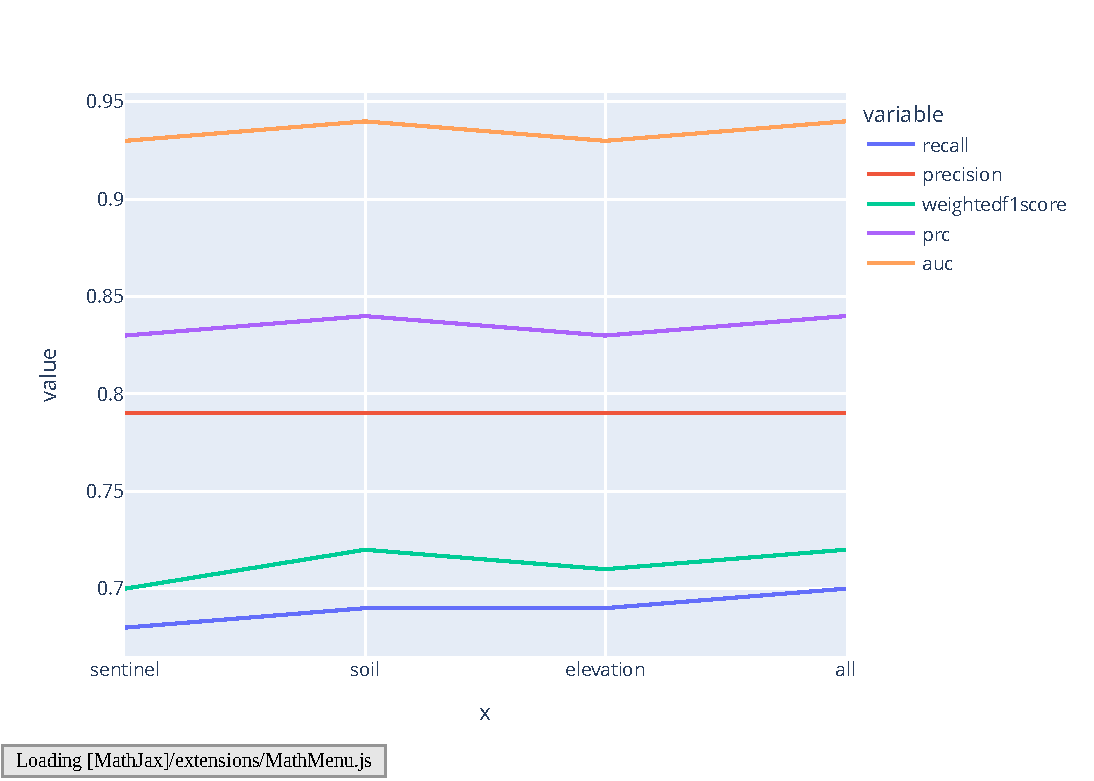
\includegraphics[width=0.9\linewidth, trim={20pt 40pt 10pt 30pt}, clip]{../report/figures/figures_analysis/soil_elevation_analysis.pdf}
\end{frame}

\begin{frame}
\frametitle{Neural Network Configuration I}
\begin{itemize}
    \item Initial hyperparameter tuning
    \item Parameters and their impact
    \item Results from Hyperband trials
\end{itemize}
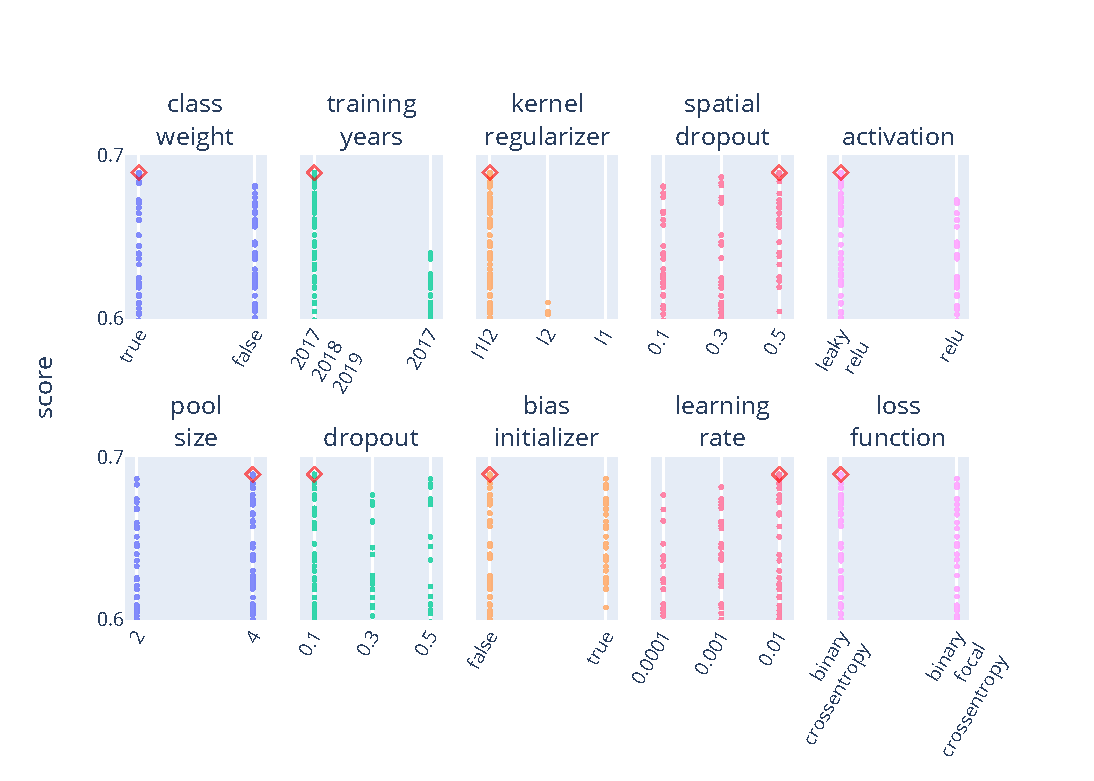
\includegraphics[width=0.9\linewidth, trim={10pt 10pt 15pt 40pt}, clip]{../report/figures/figures_tuner/hyperband_resnet_params.pdf}
\end{frame}

\begin{frame}
\frametitle{Neural Network Configuration II}
\begin{itemize}
    \item Follow-up hyperparameter tuning
    \item Optimization of layers and units
    \item Optimal configurations for performance
\end{itemize}
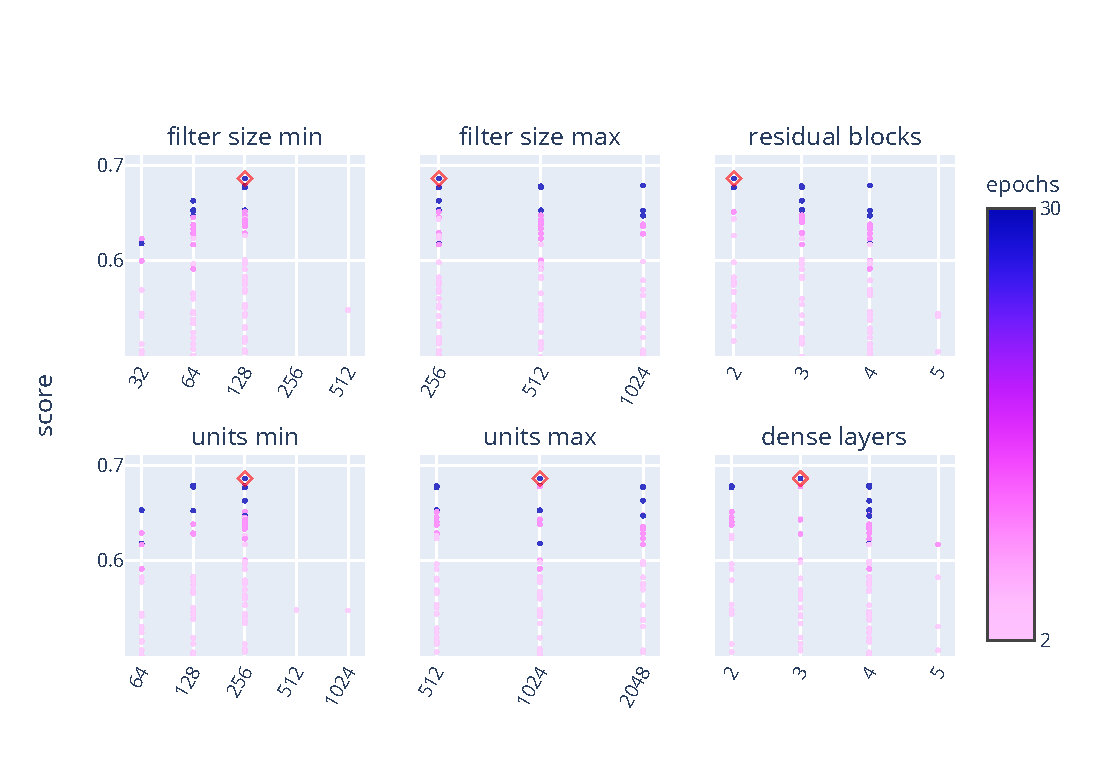
\includegraphics[width=0.9\linewidth, trim={10pt 20pt 15pt 40pt}, clip]{../report/figures/figures_tuner/hyperband_resnet_followup_params.pdf}
\end{frame}

\begin{frame}
\frametitle{Model Architecture}
\begin{itemize}
    \item Overview of model layers
    \item Convolutional and fully-connected layers
    \item Use of residual connections
\end{itemize}
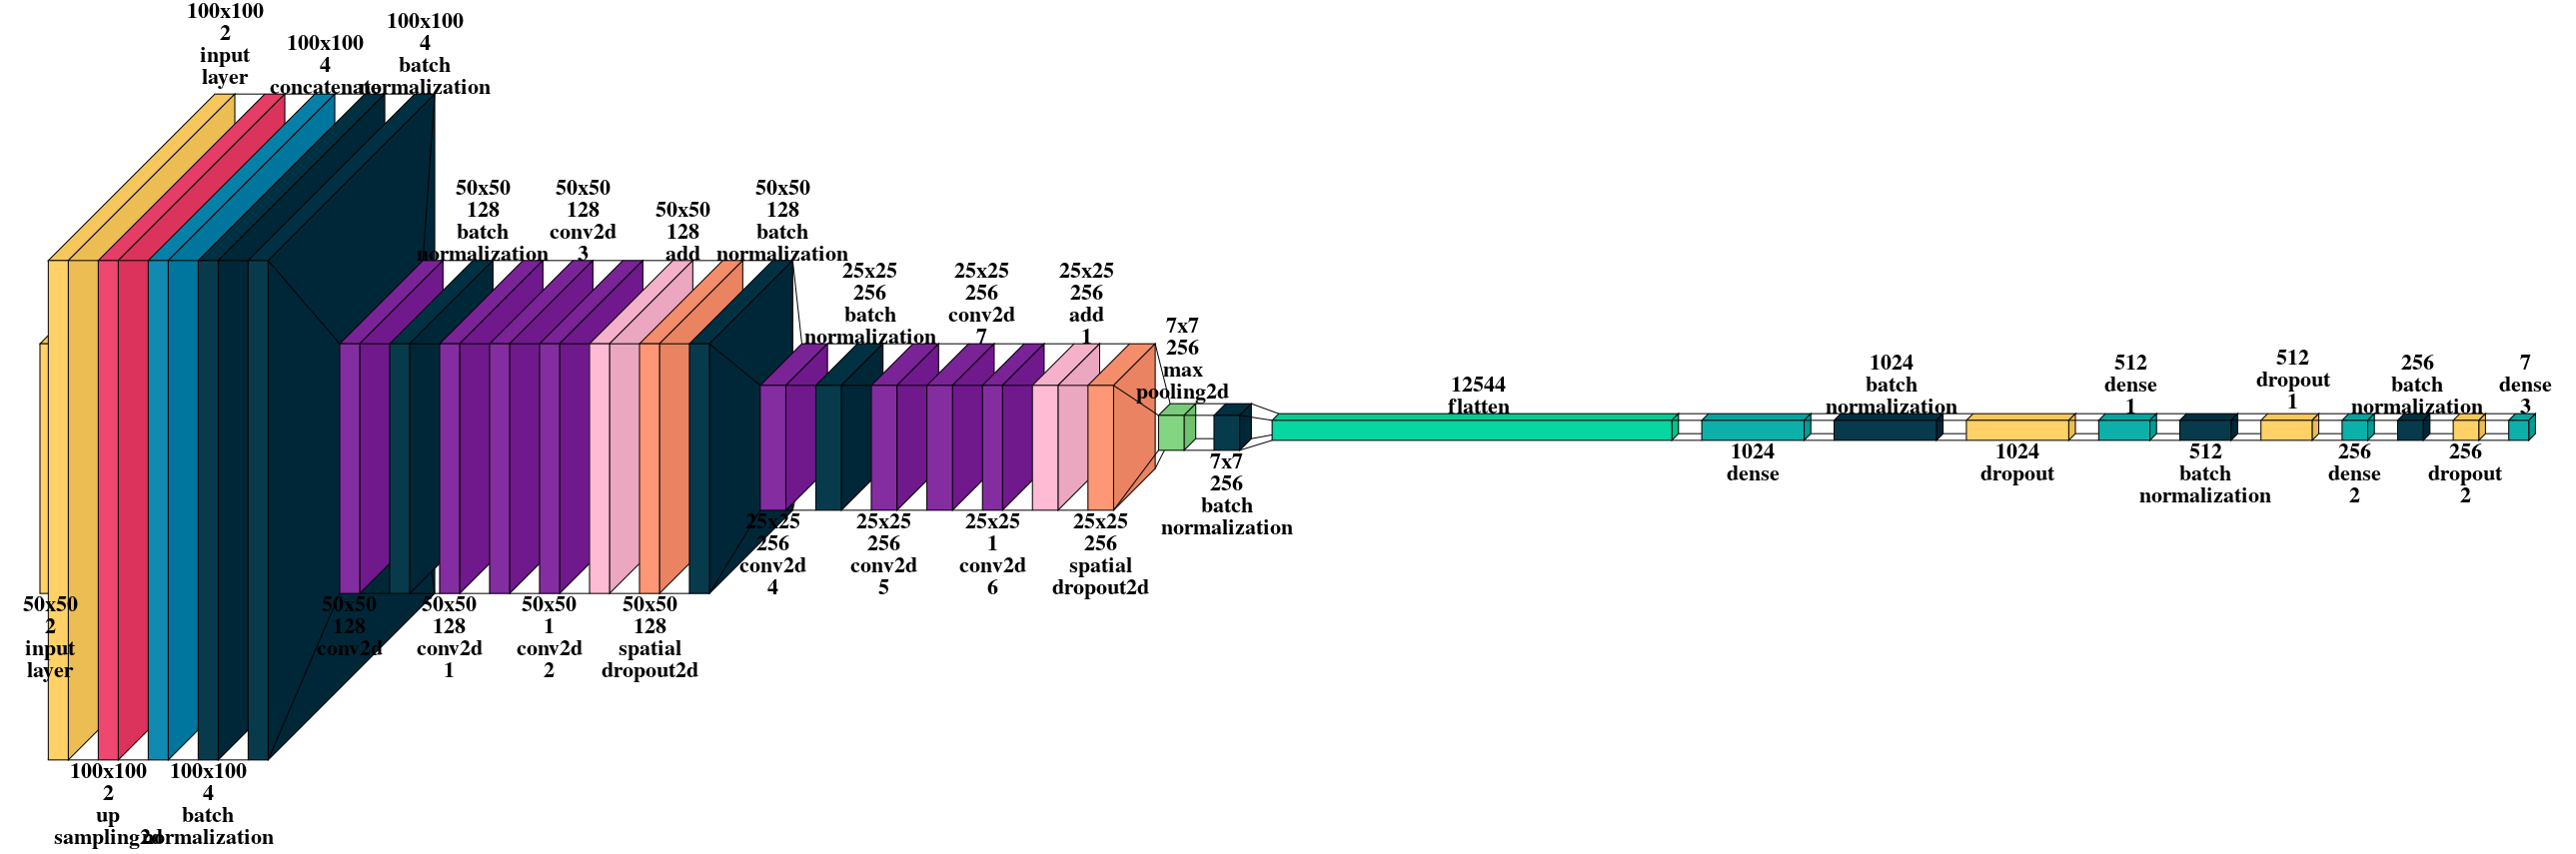
\includegraphics[width=0.99\linewidth]{../report/figures/figures_tuner/model_layered_view_together.png}
\end{frame}

\begin{frame}
\frametitle{Dataset Exploration}
\begin{itemize}
    \item Description and significance of ERA5 data
    \item Variables considered: temperature, precipitation, soil moisture
    \item Summary of selected variables
\end{itemize}
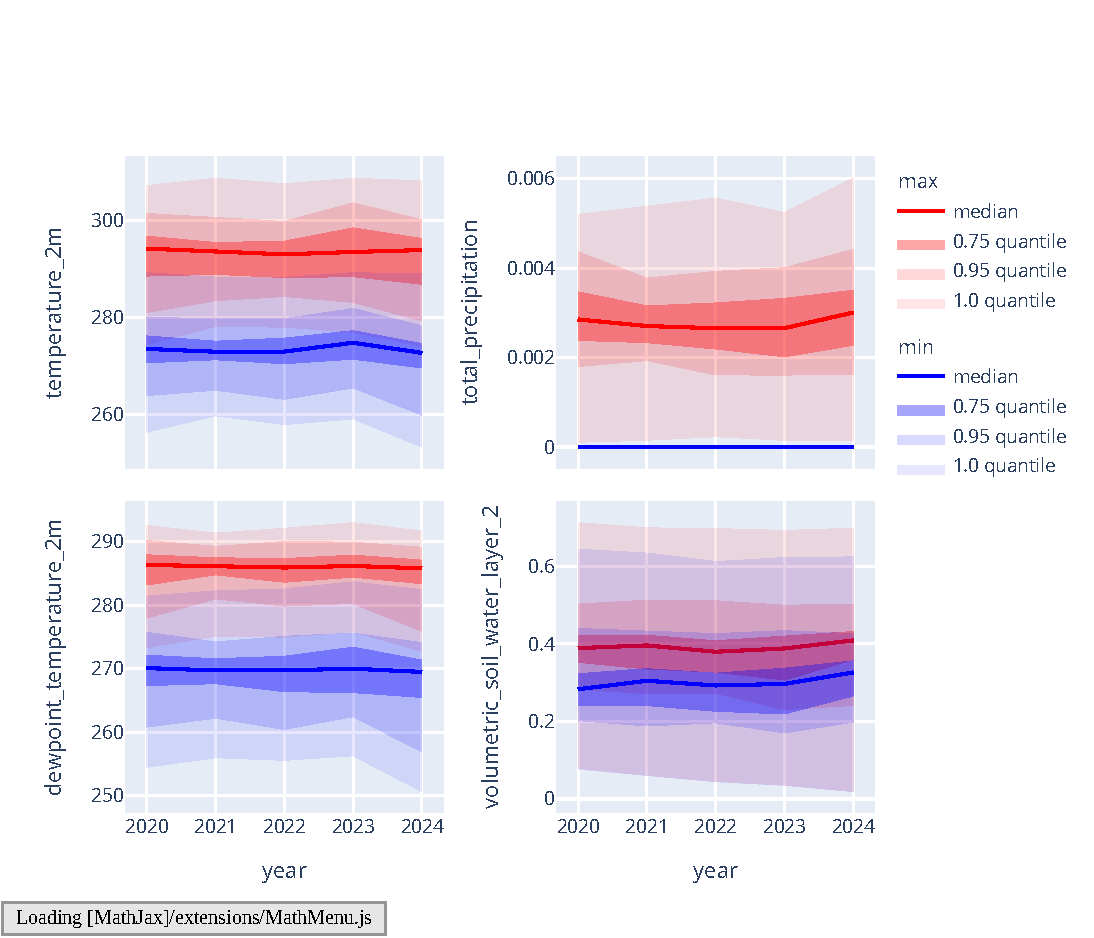
\includegraphics[width=0.8\linewidth]{../report/figures/figures_climate/selected_variables_stats.pdf}
\end{frame}

\begin{frame}
\frametitle{Class Analysis and Validation}

\begin{itemize}
    \item Classification performance varies across tree genera.
    \item Genera with fewer training samples exhibit poorer performance.
    \item Positive correlation between the number of training samples and accuracy.
\end{itemize}

\begin{figure}
    \centering
    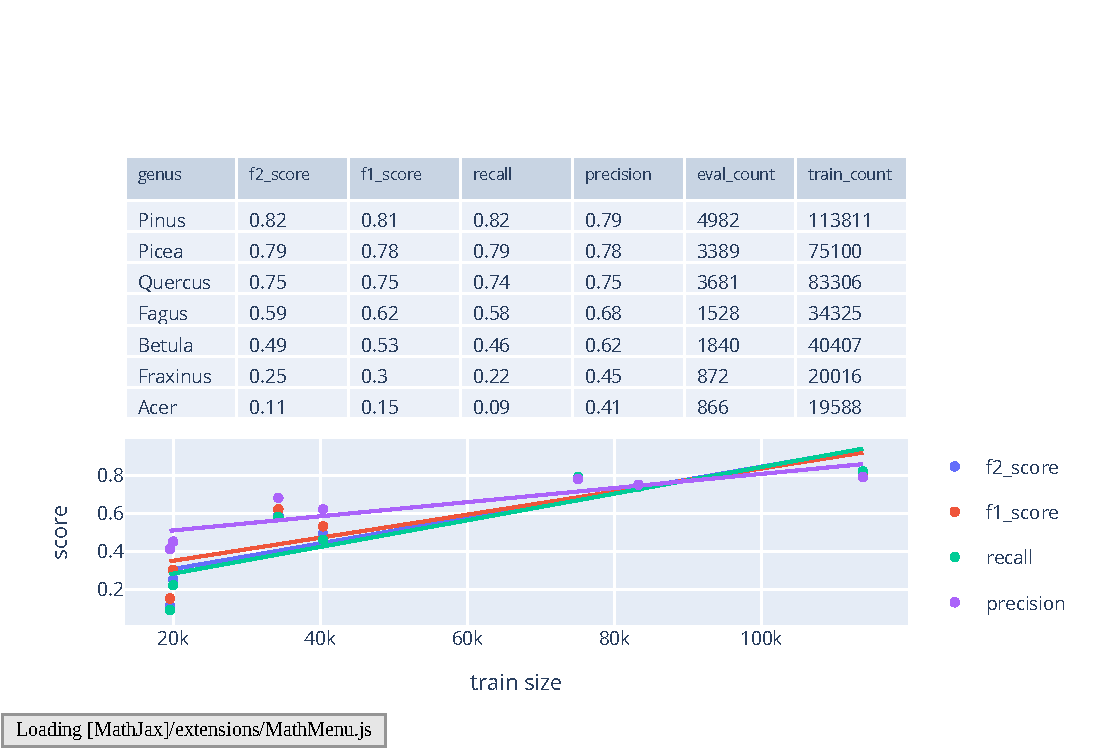
\includegraphics[width=0.9\linewidth, trim={10pt 20pt 10pt 40pt}, clip]{../report/figures/figures_class/class_analysis.pdf}
\end{figure}

\end{frame}

\begin{frame}
\frametitle{Change Map Correlations}
\begin{itemize}
    \item Correlation between tree genus changes and meteorological differences
    \item Short-term vs. long-term impacts of climate change
\end{itemize}
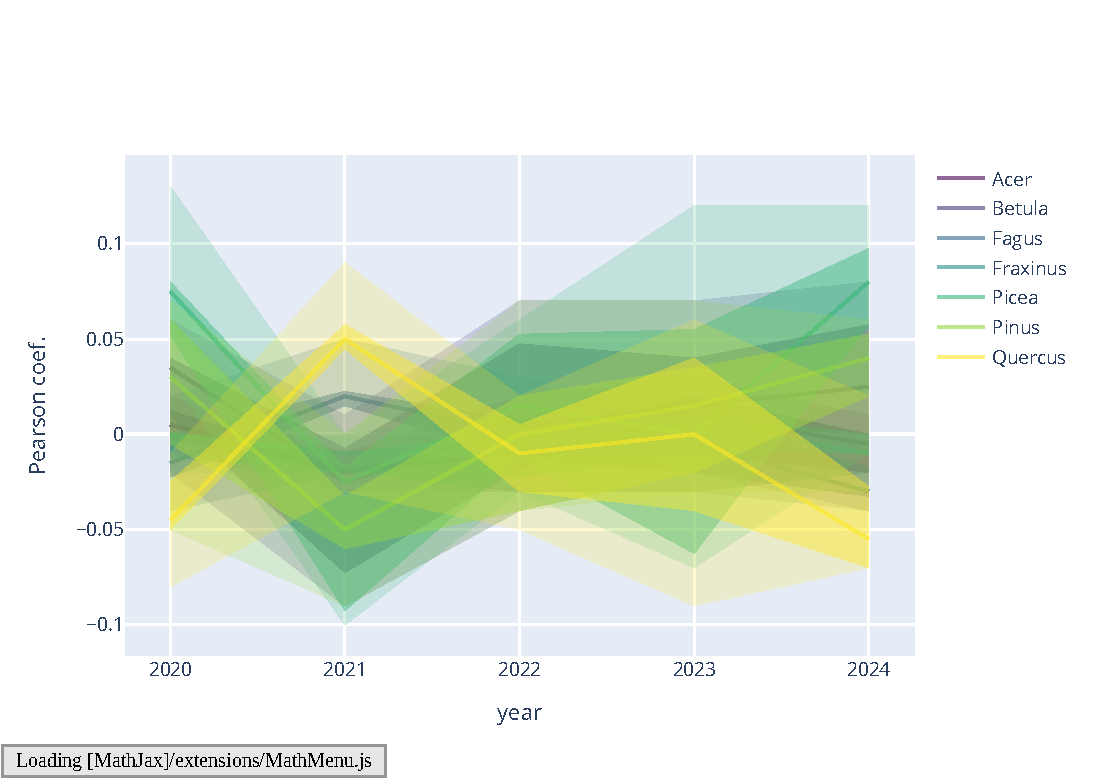
\includegraphics[width=0.9\linewidth]{../report/figures/figures_climate/genus_corr.pdf}
\end{frame}

\begin{frame}
\frametitle{Relationship Modeling}
\begin{itemize}
    \item Regression model to analyze climate-tree genus relationships
    \item Metrics: R² and MAE
    \item Model performance and results
\end{itemize}
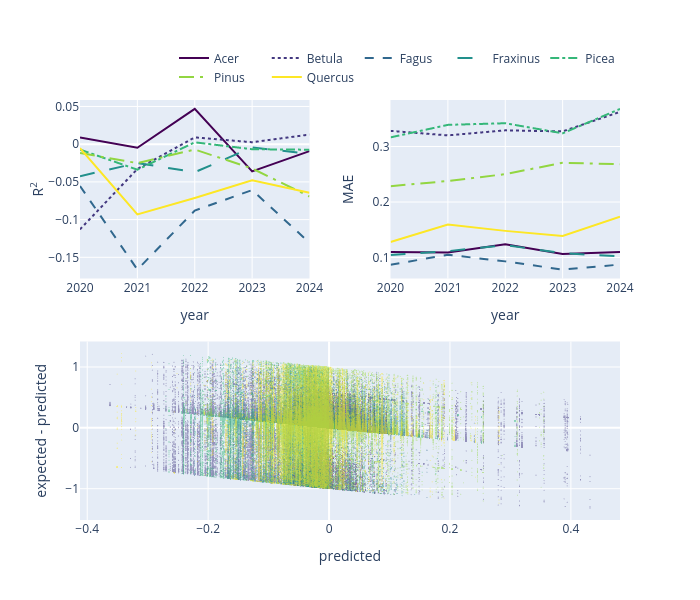
\includegraphics[width=0.8\linewidth]{../report/figures/figures_climate/regression_results.png}
\end{frame}

\begin{frame}
\frametitle{Summary and Conclusions}
\begin{itemize}
    \item Key findings from classification and climate data analysis
    \item Model performance and limitations
    \item Implications and future research directions
\end{itemize}
\end{frame}

\end{document}
